\documentclass{article}
\usepackage{graphicx}
\usepackage{wrapfig}
\usepackage{xcolor}
\usepackage{hyperref}
\usepackage{multicol}

\setlength{\textheight}{21cm}
\setlength{\textwidth}{150mm}
\setlength{\topmargin}{-2cm}
\setlength{\evensidemargin}{13mm}
\setlength{\oddsidemargin}{6mm}
\definecolor{my_col}{RGB}{25,107,200}
\pagenumbering{gobble}

\sffamily

\begin{document}

\begin{center}
	\textit{\Huge Curriculum Vitae}   
	\vspace*{1cm}
\end{center}

\begin{wrapfigure}{r}{0.25\textwidth} 
	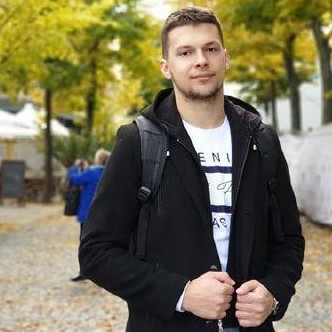
\includegraphics[width=0.27\textwidth]{my_pic.jpeg}
\end{wrapfigure}

\textbf{\large PERSONAL INFORMATIONS}\\
\color{my_col}\noindent\rule{10cm}{0.8pt}\color{black}\\ \\
Names:  \textbf{\emph{Predrag MITIC}} \\
Adress: \emph{Vlase bb, Leskovac, Serbia }\\
Tel: 	(+381) 61 18 56 816 \\
Email	predrag98mitic@gmail.com \\ 
Web:	\url{www.alas.matf.bg.ac.rs/~mi17116} \\
Github:	\url{www.github.com/PredragMitic} \\ 
Date of Birth: 1/09/1998 \\ \\

\textbf{\large PERSONAL PROFILE}\\
\color{my_col}\noindent\rule{15.4cm}{0.6pt}\color{black}\\ 
Ambitious and highly motivated third year student at Faculty of Matematics, 
University of Belgrade. With practical experiance in Computer Graphics and 
C/C++ programming language. Team player, quick learner, open to new ideas and experiances.\\

\textbf{\large KEY SKILLS AND ACHIVEMENTS}\\
\color{my_col}\noindent\rule{15.4cm}{0.6pt}\color{black}
\normalsize
\begin{itemize}
  \item Good at solving algorithm problems
  \item Extensive knowledge of programing and programming languages 
  (C/C++, Java, Python, JavaScript, SQL, R, MATHLAB)
  \item Good knowledge of text markup languages (HTML/CSS, LaTeX)
  \item Competent user of Microsoft Office, Autodesk softwre, 
  Linux OS and Microsoft Windows OS
  \item Excellent in 3D and 2D graphics 
  \item Languages:
	\begin{itemize}	\small
		\item Serbian - Native
		\item English - B1+
		\item German - A1
	\end{itemize}
\end{itemize}

\begin{description}
    \item[ 2016] - Fourth place in 3D Computer Grapics (Autodesk Inventor)\\
    National Competition
    \item[ 2016] - Second place in Electronics\\
    National Competition
    \item[ 2015] - First place in 2D Computer Grapics (Autodesk AutoCAD)\\
    Regional Competition
    \item[ 2014] - First place in 2D Computer Grapics (Autodesk AutoCAD)\\
    National Competition
\end{description}

\textbf{\large EDUCATION}\\
\color{my_col}\noindent\rule{15.4cm}{0.6pt}\color{black}
\begin{description}
    \item[ 2017-2021 : Bachelor of Informatics ]\hfill \\
    \textbf{\textit{Faculty of Mathematics, University of Belgrade}}\\
    \normalsize \\
    Subjects stuied :
     \begin{multicols}{2}
    \begin{itemize}
    \item Programming
    \item Computer Architecutre
    \item Algorithms and Data structures
    \item Operating Systems
    \item Database Systems
    \item Web programming
    \item Geometry
    \item Numerical Mathematics
    \item Probability and Statistics 
    \item English
    \end{itemize}
    \end{multicols}
\end{description}

\begin{description}
    \item[ 2013-2017 : Mechatronics Technician] GPA(5.00/5.00)\hfill \\
    \textbf{\textit{Technical School, Leskovac}}\\
    \normalsize \\
    Subjects stuied :
     \begin{multicols}{2}
    \begin{itemize}
    \item Mathematics
    \item Programming (C, C++, PLC)
    \item Electrical engineering and Electronics
    \item Mechanical engineering
    \item Automatic Systems
    \item English
    \end{itemize}
    \end{multicols}
\end{description}


\textbf{\large EMPLOYMENTS AND TRAININGS}\\
\color{my_col}\noindent\rule{15.4cm}{0.6pt}\color{black}
\begin{description}
    \item[ 2019] - RT-RK Summer School \\
    \textit{Modern Improvments in C++}
   
\end{description}

\textbf{\large INTERESTS}\\
\color{my_col}\noindent\rule{15.4cm}{0.6pt}\color{black}\\
Algorithm and Data Structures, Computer Graphics, Database Systems, 
C++ Programming, Artificial Intelligence, foregin languages and travel\\

\textbf{\large PROJECTS}\\
\color{my_col}\noindent\rule{15.4cm}{0.6pt}\color{black}
\begin{description}
    \item[ C/OpenGL] - Shoot Training\\ 
    Game made in C program language and OpenGl(Open Graphics Library)
    \item[ HTML/NodeJS] - Web Library\\ 
    Web page for online library powered by NodeJS
\end{description}
My projects can be seen on my Github profile \\
%\textbf{\large REFRERENCIS}\\
%\color{my_col}\noindent\rule{15.4cm}{0.6pt}\color{black}\\ 

\color{my_col}\noindent\rule{15.4cm}{0.6pt}\color{black}\\
\textbf{\large Belgrade, 31/12/2019}\\






\end{document}
